% Preamble
\documentclass[12pt, a4paper]{article}

% Packages
\usepackage{graphicx}
\usepackage{float}
\usepackage[nottoc]{tocbibind}
\usepackage[tablegrid]{vhistory}
\usepackage{enumitem} 
\usepackage{url}
\usepackage{listings}
\usepackage[hidelinks]{hyperref}
\usepackage{fancyhdr}
\usepackage[paper=a4paper, margin=2.5cm]{geometry}
\usepackage{titlesec}	

\def \version {1.0}

% Settings

\hypersetup
{
	pdfauthor={Gijs Alberts, Anne Zweers},
	pdfsubject={Report on Final Assignment},
	pdftitle={Report on Final Assignment - v\version},
	pdfkeywords={Final Assignment, Game AI, Report}
}

\parindent 0 pt 
\title{Report on Final Assignment - v\version}
\date{\today}
\author{Gijs Alberts \\ Anne Zweers}
\rhead{Report v\version}
\lhead{Report - Final Assignment - Game AI}
\rfoot{Page \thepage}
\pagenumbering{arabic}
\graphicspath{ {Images/} }
\setlength{\parindent}{0em}

% Document
\begin{document}
	\newgeometry{margin=1.1cm, lmargin=1.4cm, top=2cm}
	\begin{titlepage}
		
		
		\LARGE Report - Final Assignment v\version \\
		\huge Game AI. \hfill
		\vspace{0.5cm}
		
		\small HBO-ICT, Games Programming \\
		Windesheim University of Applied Sciences \\
		Lecturer: Gido Hakvoort
		\begin{center}
			\vspace{4cm}
			\hspace*{-1.0cm}\textsl{}
			\makebox[\textwidth]{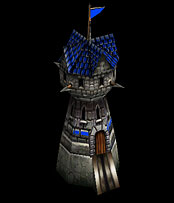
\includegraphics[width=300pt]{Images/coverpage_logo.jpg}}
		\end{center}
		\vfill
		\normalsize
		Windesheim, Zwolle \\
		Version: \version \\
		\today \\
		Authors : Gijs Alberts, Anne Zweers \\
	\end{titlepage}
	\restoregeometry
	\thispagestyle{empty}
	\newpage
	\begin{versionhistory}
		\vhEntry{1.0}{12-04-2018}{ Gijs Alberts \newline Anne Zweers}{Initial version of the document.}
	
	\end{versionhistory}
	\thispagestyle{empty}
	\newpage
	\setcounter{page}{1}
	\tableofcontents
	\newpage
	\section{Introduction}\label{sec:intro}
	\subsection{Tussenkopje}
citatie van iets \cite{gitlabwebsite} 
zie voor bibid bibliography in FinalAssignment
\subsubsection{tussentussenkopje}
\paragraph{paragraaf}
\subparagraph{subparagraaf} 


	\newpage
	\section{Steering}\label{sec:steering}
	In this chapter we will describe: 
\begin{itemize}
	\item The steering behaviors we implemented.
	\item How we implemented these steering behaviors.
	\item The issues and problems we faced while implementing the steering behaviors and how we solved these issues.
	\item How steering behaviors can be combined within our game.
\end{itemize}
A class diagram about all of the classes that are relevant to the steering behaviors can be found at the bottom of this chapter.
\subsection{Behaviors}
We implemented the following steering behaviors: 
\begin{itemize}
	\item Seek. \\ 
	Will steer the agent towards a target within the game.
	\item Flee. \\
	Will steer the agent away from a target within the game.
	\item Arrive. \\
	Will steer the agent towards a target within the game and will decelerate as the agent gets closer to the target position.
	\item Follow Path. \\ 
	Will steer the agent along a path. 
	Uses seek to reach all the waypoints but the last waypoint within the path. 
	Arrive is used for the last waypoint.
	\item Pursuit. \\
	Will steer the agent towards a target agent.
	\item Evade. \\ 
	Will steer the agent away from a target agent.
	\item Offset Pursuit. \\
	Will steer the agent towards a target agent while keeping a distance between them.
	\item Explore. \\
	Will make the agent explore a queue of Powerups.
\end{itemize}
Our implementation supports the following summing methods: 
\begin{itemize}
	\item Weighted truncated sum.
	\item Prioritization.
	\item Prioritized dithering.
\end{itemize}
\subsection{Issues and Solutions}
We mainly just rewrote the source from the Programming Game AI by Example book by Mat Buckland into C\# so we didn't have too many problems. We had some issues with updating the Velocity/Heading of the agent's and calculating the steering force based on the elapsed time. The measurement of elapsed time that Mat Buckland uses didn't seem to be documented within the source so it took some adjustments to get it about right. \\\\ We used a different implementation for the Offset Pursuit than the book did. The reason for this is that this seemed like a simpler implementation with the same effect.

\begin{figure}[H]
	\centering
	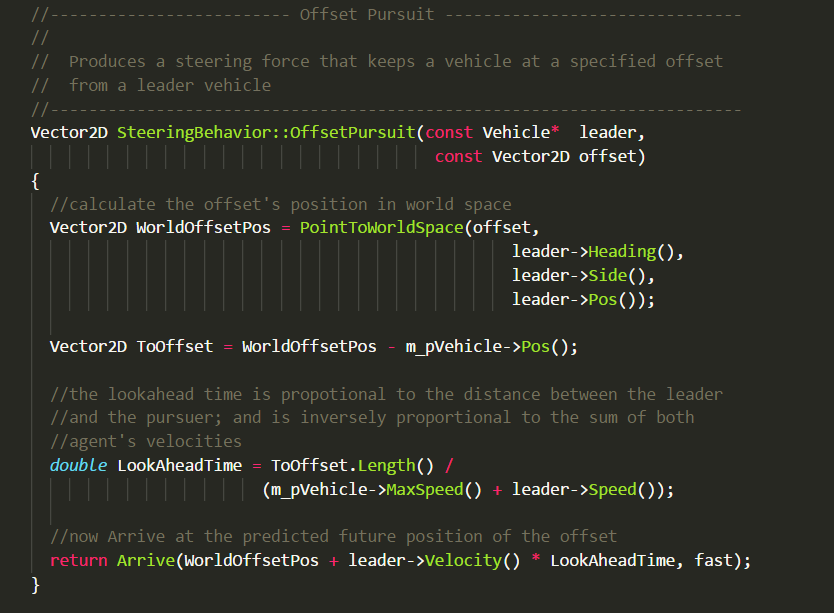
\includegraphics[width=0.7\linewidth]{Images/offsetsource}
	\caption{Original Offset Pursuit.}
	\label{fig:offsetimplementation}
\end{figure} 
\begin{figure}[H]
	\centering
	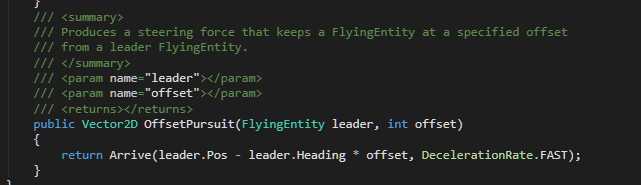
\includegraphics[width=0.7\linewidth]{Images/offsetimplementation}
	\caption{Implementation of Offset Pursuit.}
	\label{fig:offsetsource}
\end{figure} 
We also had some issues with oscillation which were solved by creating a threshold.
We basically made it so that if the agent is within a certain very close distance to the target position the agent's position will be transformed into the target position after finding an article about the issue. \cite{steeringissue}. 
\subsection{Combining Steering Behaviors}
Combining multiple steering behaviors is very easy since we use a bit operator system for it (just like the book did). 
\begin{figure}[H]
	\centering
	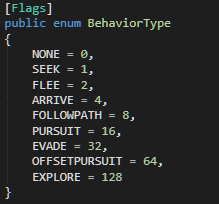
\includegraphics[width=0.7\linewidth]{Images/bitoperatorsflagenum}
	\caption{Behaviour flags.}
	\label{fig:behaviourflags}
\end{figure} 
\begin{figure}[H]
	\centering
	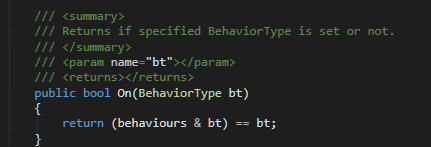
\includegraphics[width=0.7\linewidth]{Images/bitoperatorson}
	\caption{Method for asserting if a behavior is enabled or not.}
	\label{fig:offsetsource}
\end{figure} 
\begin{figure}[H]
	\centering
	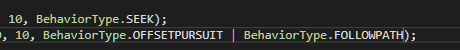
\includegraphics[width=0.7\linewidth]{Images/multiplebehaviors}
	\caption{Combining steering behaviors.}
	\label{fig:multiplebehaviors}
\end{figure}

\subsection{Class Diagram}
\begin{figure}[H]
	\centering
	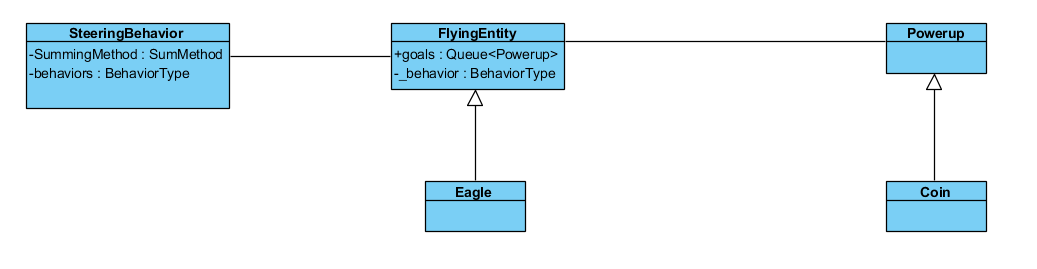
\includegraphics[width=0.7\linewidth]{Images/steeringclassdiagram}
	\caption{Class diagram of classes that are relevant to steering.}
	\label{fig:steeringclassdiagram}
\end{figure}
	\newpage
	\section{Path Planning}
	In this chapter we will describe: 

\begin{itemize}
	\item How the graph representing the environment is generated.
	\item The heuristic we use in A*.
\end{itemize}

A class diagram about all of the classes that are relevant to the path planning can be found at the bottom of this chapter.
	\newpage
	\section{Behavior}
	\input{Sections/Behavior}
	\newpage
	\section{Fuzzy Logic}
	\input{Sections/FuzzyLogic}
	\newpage
	\section{Conclusion}\label{sec:planning}
	We would like to think we did ok for this project, although there are many things that could be improved upon. \\\\ Some examples of what we think could be improved upon are the implementation of fuzzy logic. We currently have strangely formed FLV's that do however seem to work. When changing the graphs to be a normal format we have a bug where the defuzzification of the distance to the enemy always seems to return 0 and therefore we decided to keep the graphs the way they were. \\\\ We also think the enemy/entity implementation we have could be improved on. We only later discovered the source found within the book and we already had the enemy-hierarchy implemented. after that we decided to implement the entity-hierarchy like the book did but the combination of both creates awkward situations such as the eagle not being an Enemy. \\\\ We think the main difficulties we had with the project were finding about the book source too late and partly because of that, not being ready for the deadline. After the deadline we both were quite busy with the game project and had to work on the Tower Defense game during the weekends mainly which isn't a great excuse but it lead to us taking so long to hand this in. \\\\ On the more positive side we think we implemented most required features or atleast tried to implement them, We feel like we have some good parts within the code unlike the enemy-entity system. Such as the Powerup hierarchy for the explore and being able to specify a Queue of Powerups for the Flying Entity to explore, it would be very easy to expand this to include different kinds of Powerups. We also think we did a decent job on commenting the code and staying consistent with our conventions.
	\newpage
	\appendix
	\begin{thebibliography}{9}
		\bibitem{gitlabwebsite} 
	  	\textit{GitLab: Issue Board}.
	  		\\\textit{\url{https://docs.gitlab.com/ee/user/project/issue_board.html}}
	  
	\end{thebibliography}
\end{document}          